% =====================================================================
%  chunks/ch04c.tex —— 原书 p.165–175（PDF 172–182）
%  第 4 章 §2 光滑流形的同调论。复流形。经典整体变分法。
%  $H$ 空间。多值函数与泛函（上）
% =====================================================================
% [原文 p.165]
最简单的紧复流形是复射影空间 $\CP^n$，以及偶维环面 $T^{2n}=\C^n/\Gamma$，其中 $\Gamma$ 是由 $\C^n\cong\R^{2n}$ 中任意 $2n$ 个线性无关实向量张成的格。特别重要的是紧复子流形 $M^k\subset\CP^n$，即射影代数簇。

复流形 $M^n$ 上的 \emph{Hermitian 度量}用各坐标卡 $V_\alpha$ 上的局部坐标给出：
\[
  ds^2=g_{ij}\,dz_\alpha^i\,d\bar z_\alpha^j,\qquad g_{ij}=\bar g_{ji}.
\]
借助这样的度量，可以配出一个实 2-形式，它局部地写成
\[
  \Omega=\frac{\ii}{2}\,g_{ij}\,dz_\alpha^i\wedge d\bar z_\alpha^j.
\]
要求切向量沿任意道路的平行移动都给出酉变换，便导致 2-形式 $\Omega$ 闭：
\[
  d\Omega=0.
\]
带有 Hermitian 度量、且其相配 2-形式 $\Omega$ 闭的复流形称为 \emph{Kähler 流形}。若 Kähler 流形 $M^n$ 上的形式 $\Omega$ 表示一个整上同调类，即 $\Omega$ 在 $M^n$ 中任意 2-闭链上的积分取整数值，则称 $M^n$ 为 \emph{Hodge 流形}。复射影空间 $\CP^n$ 及其复子流形（代数簇）都是 Hodge 流形。事实上，每个 Hodge 流形都是射影代数簇；这一点对复环面由 Siegel 证明，一般情形由 Kodaira 在 20 世纪 40 年代末证明。赋以分量 $g_{ij}$ 为常数的 Hermitian 度量的复环面是 Kähler 流形，但它是复射影代数簇当且仅当定义格 $\Gamma\subset\C^n$ 满足 Riemann 条件，使相应的 $\theta$ 函数可以定义。

$\C^n$ 中无边界、维数 $>0$ 的复子流形都是非紧的。关于复流形拓扑的进一步结果将在后面几节给出。
% [Tutor Note: $\Omega$ 前乘以因子 $\ii/2$ 正是为了使它成为实 2-形式：由 $g_{ij}=\bar g_{ji}$ 可验证 $\bar\Omega=\Omega$。$\Omega$ 称为 Kähler 形式；$d\Omega=0$ 等价于度量的 Hermitian 联络无挠。]

\section[光滑流形的同调论。 复流形。 经典整体变分法。 H 空间。 多值函数与泛函]{光滑流形的同调论。复流形。经典整体变分法。$H$ 空间。多值函数与泛函}
\takeaway{本节把单纯同调与上同调的整套机器（杯积、相交、Poincaré 对偶）搬到光滑流形上，再讨论复流形上的 Hermitian 度量、Kähler 流形与 Hodge 流形，以及经典整体变分法、$H$ 空间与多值函数。核心工具是光滑三角剖分与一般位置的横截相交。}

光滑类为 $C^k$、$k\ge 1$ 的每个可微流形 $M^n$ 都可三角剖分，即化为单纯复形。一个\emph{光滑单形}是一对数据：标准单形 $\sigma^k\subset\R^k$，以及某个 $k$ 维开区域 $U$（$\sigma^k\subset U\subset\R^k$）到流形的正则光滑嵌入
\[
  f_k:U\longrightarrow M^n.
\]
% [原文 p.166]
于是 $M^n$ 的\emph{光滑三角剖分}就是把 $M^n$ 单纯分解为光滑单形：
\[
  M^n=\bigcup_{\alpha,k}f_{k,\alpha}(\sigma^k),
\]
它使 $M^n$ 成为一个「PL 流形」，即：由包含任一给定单形的全部单形构成的单纯复形，与标准 $n$-单形 $\sigma^n$ 组合等价（见第 3 章 §1）。

在组合等价的意义下，任一光滑流形 $M^n$ 只有一个光滑三角剖分（Cairns、Whitehead，20 世纪 30 年代）。因此，单纯同调与上同调的标准机器（$H_*(M^n)$、$H^*(M^n)$、使 $H^*$ 成为环的乘法、$H_*(M^n)$ 中闭链的相交、Poincaré 对偶等等——见第 3 章 §1、§2）经由光滑三角剖分整体地搬到光滑流形 $M^n$ 上（见图 4.6）。

\begin{figure}[htbp]
  \centering
  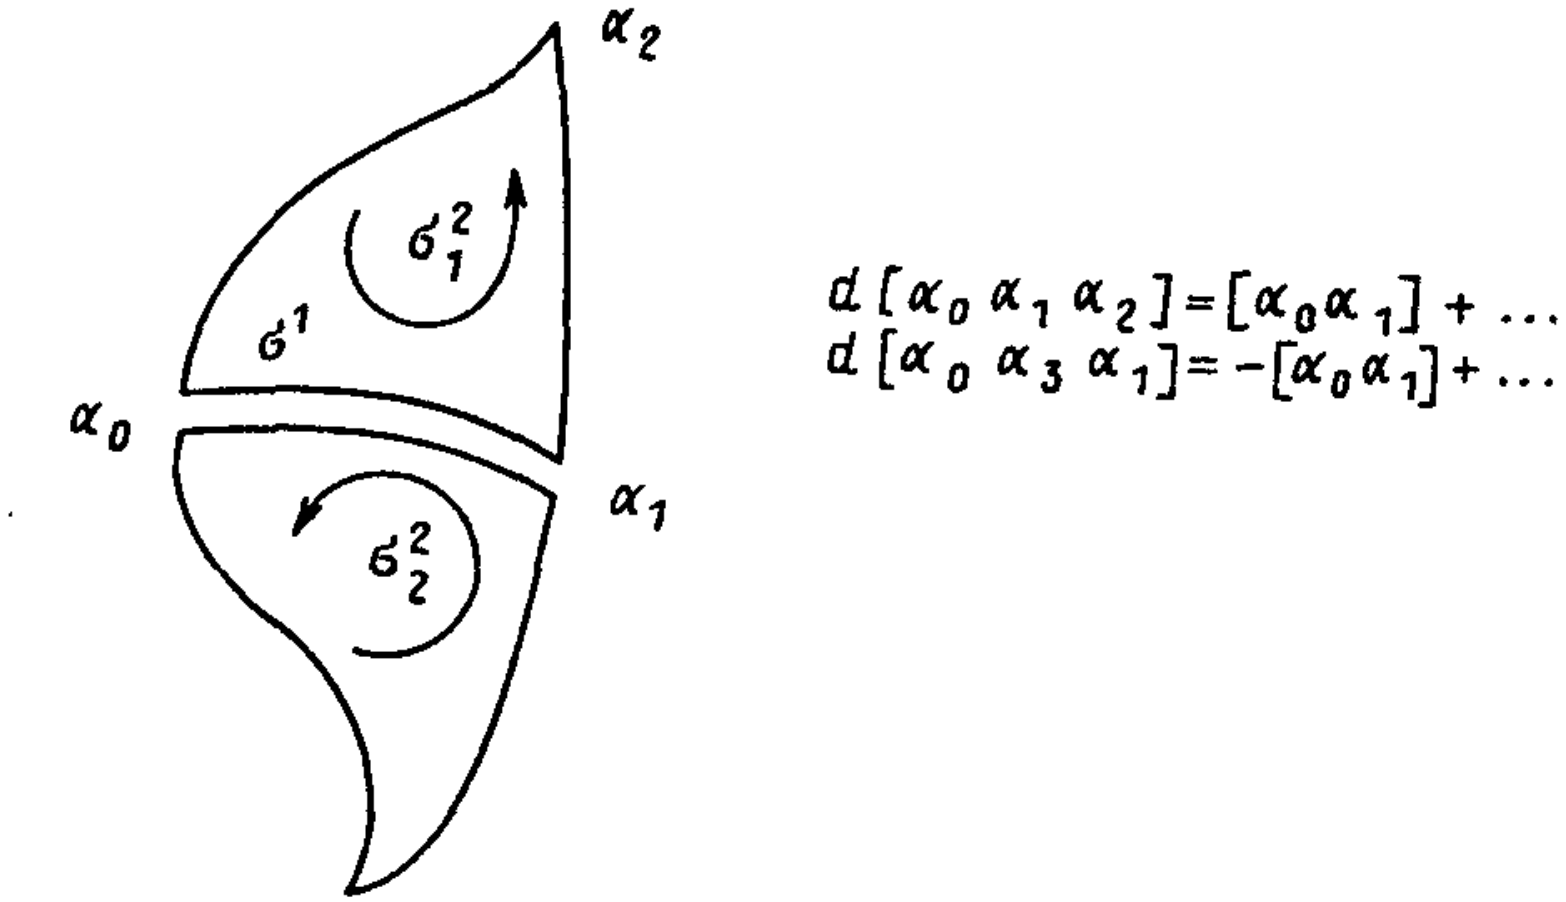
\includegraphics[width=0.62\textwidth]{figures/fig4_6.png}
  \figtitle{4.6}{}
\end{figure}

对闭子流形 $W^k,V^j\subset M^n$，相交运算有清晰的几何解释。先对 $W^k$ 作任意小的扰动，使它相对于 $V^j$ 处于「一般位置」：对每一点 $x\in W^k\cap V^j$，切于 $W^k$ 或 $V^j$ 的向量合起来张成外围流形 $M^n$ 在 $x$ 处的整个切空间 $\R^n_x$。于是若 $k+j<n$，一般位置下的交 $W^k\cap V^j$ 为空。若 $k+j=n$，则（一般位置下的）交由有限多个孤立点 $x_1,\dots,x_m$ 组成（见图 4.7）；此时这些点的个数 $m$ 模 2 给出模 2 相交指数：
\begin{equation}
  W^k\circ V^j\equiv m\ (\mathrm{mod}\ 2). \tag{2.1}
\end{equation}
若流形 $M^n$、$W^k$、$V^j$ 都带定向，则交 $W^k\cap V^j$ 的每一点 $x_j$ 都附有一个符号 $\sgn_{x_j}(W^k\cap V^j)$：它是从与 $M^n$ 的给定定向相符的、$M^n$ 在 $x_j$ 处切空间的标架 $\tau_{x_j}$，变到标架 $(\tau'_{x_j},\tau''_{x_j})$ 时过渡矩阵行列式的符号；其中 $\tau'_{x_j}$ 是 $W^k$ 在 $x_j$ 处与 $W^k$ 的给定定向相符的切标架，$\tau''_{x_j}$ 类似地是相对于 $V^j$ 的切标架。于是
\begin{align}
  W^k\circ V^j &= \sum_j\sgn_{x_j}(W^k\cap V^j), \notag\\
  V^j\circ W^k &= (-1)^{kj}(W^k\circ V^j). \tag{2.2}
\end{align}
% [原文 p.167]
对光滑可定向流形 $M^n$，可以为各群 $H^j(M^n;\Z)$（$j=0,1,\dots,n$）选取一对基
\[
  \{z_j^{\alpha_j}\},\qquad \{\tilde z_j^{\alpha_j}\},\qquad \alpha_j=1,\dots,b_j,
\]
使它们两两互为 Poincaré 对偶：
\begin{equation}
\begin{gathered}
  z_j^{\alpha_j}\circ\tilde z_{n-j}^{\alpha_{n-j}}=\delta_{\alpha_j\alpha_{n-j}},\\
  z_0=\tilde z_0=1,\qquad z_n=\tilde z_n=[M^n].
\end{gathered}\tag{2.3}
\end{equation}
当 $n=2m$ 时，特别地有群 $H^m(M^{2m};\Z)$ 的两个基 $\{z_m^{\alpha_m}\}$、$\{\tilde z_m^{\alpha_m}\}$（$\alpha_m=1,\dots,b_m$），满足
\[
  z_m^i\circ\tilde z_m^j=\delta_{ij},
\]
因而彼此 Poincaré 对偶。（对不可定向流形，存在模 2 意义下类似的对偶基。）

\begin{example}{}
设 $M^n$ 是闭可定向流形，$f:M^n\to M^n$ 是任意正则光滑自映射。考虑 $M^n\times M^n$ 中的如下闭链（对角线与 $f$ 的图像）：
\[
  \Delta=\{(x,x)\}\in H_n(M^n\times M^n;\Q);\qquad
  \Delta_f=\{(x,f(x))\}\in H_n(M^n\times M^n;\Q).
\]
上面已指出，一般位置下交 $\Delta\cap\Delta_f$ 由孤立点 $x_j$ 组成：$f(x_j)=x_j$。由于 $f$ 的正则性以及闭链 $\Delta$、$\Delta_f$ 彼此处于一般位置的假设，这些点都是非退化的，即：在点 $x_j$ 的邻域内用局部坐标 $x_a^q$ 表示，
% [原文 p.168]
\[
  \det\left(\delta_{pq}-\frac{\partial f^p}{\partial x^q}\right)_{x=x_j}\ne 0.
\]
\begin{figure}[htbp]
  \centering
  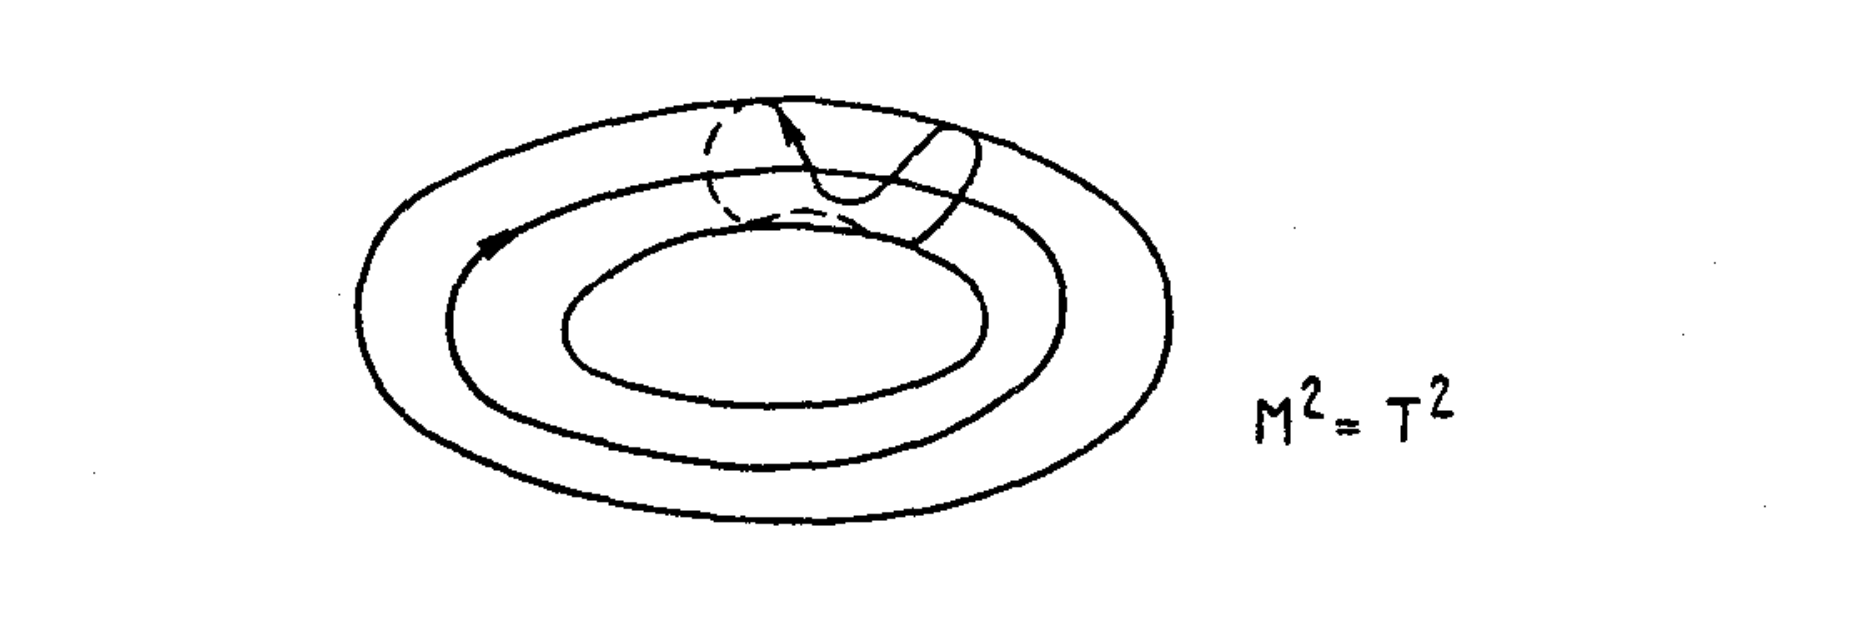
\includegraphics[width=0.55\textwidth]{figures/fig4_7.png}
  \figtitle{4.7}{}
\end{figure}
此时相交指数就是这些不动点 $x_j$ 上所附符号之和：
\begin{equation}
  \Delta\circ\Delta_f=\sum_{x_j\in\Delta\cap\Delta_f}\sgn\det
  \left(\delta_{pq}-\frac{\partial f^p}{\partial x^q}\right)_{x=x_j}. \tag{2.4}
\end{equation}
由满足式 (2.3) 的基 $\{z_j^{\alpha_j}\}$、$\{\tilde z_j^{\alpha_j}\}$，可以得到 $H_n(M^n\times M^n;\Q)$ 的基 $z_j^{\alpha_j}\otimes\tilde z_{n-j}^{\alpha_{n-j}}$，借助它并由式 (2.4) 即可建立 Lefschetz 公式（约 1920 年）
\begin{equation}
  \Delta\circ\Delta_f=\sum_{k\ge 0}(-1)^k\Tr f_*\big|_{H_k(M^n;\Q)}. \tag{2.5}
\end{equation}
由此可知：若 $f$ 零同伦，则 $\Delta\circ\Delta_f=1$。把它用于 $M^n=S^n$，并把圆盘 $D^n$ 看作 $S^n$ 的半球（$D^n\subset S^n$），便可推出 Brouwer 定理（约 1910 年）：任何映射 $D^n\to D^n$ 都有不动点。
\end{example}

\begin{figure}[htbp]
  \centering
  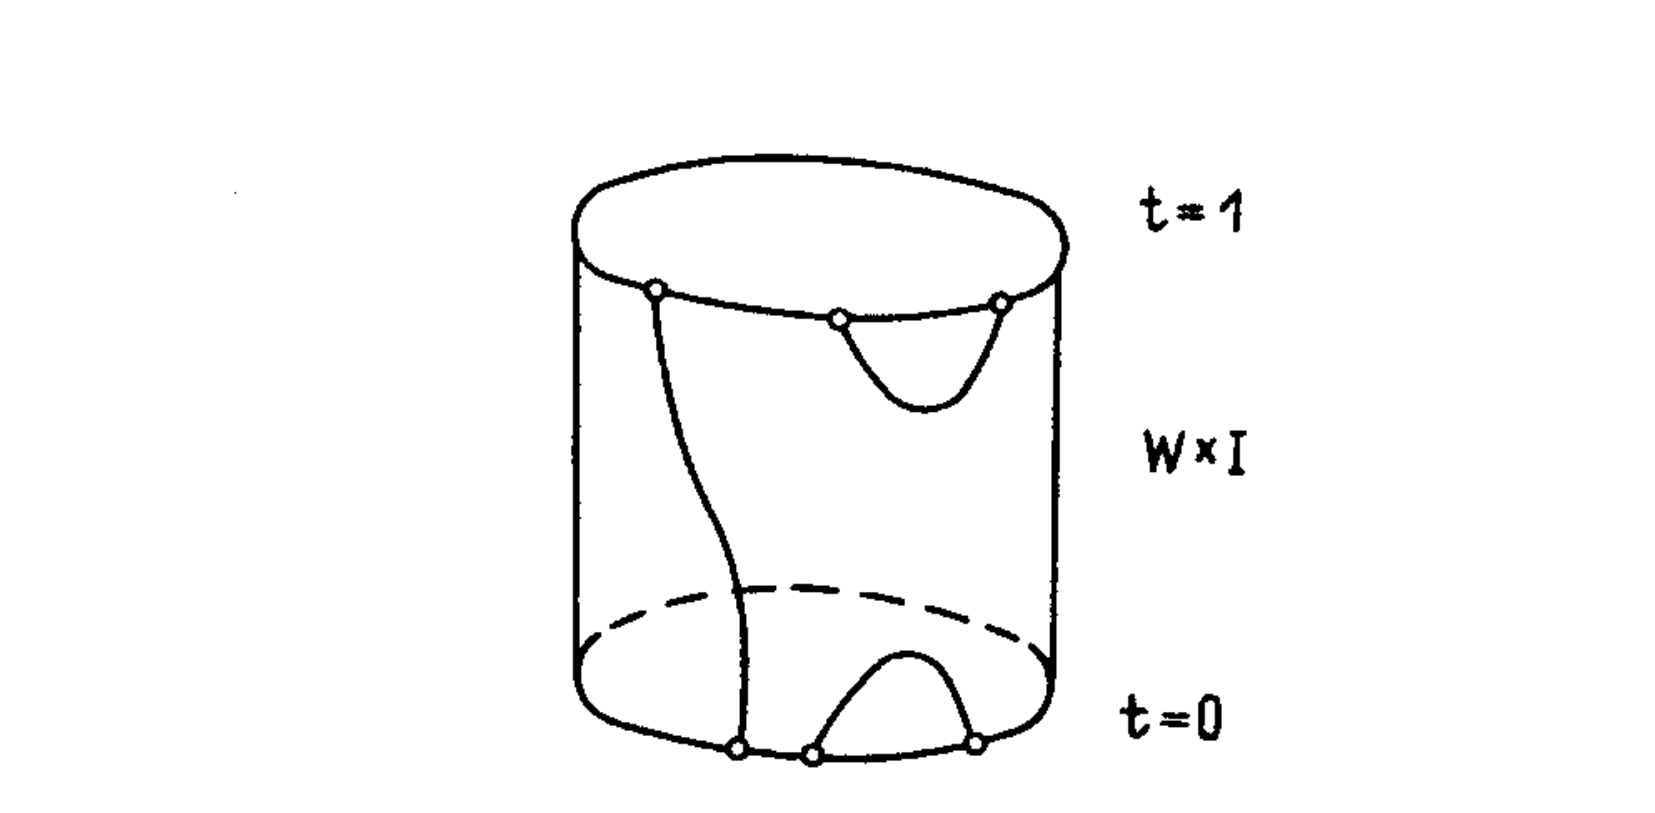
\includegraphics[width=0.55\textwidth]{figures/fig4_8.png}
  \figtitle{4.8}{相交指数在闭链形变下不变}
\end{figure}

回到闭子流形 $W^k,V^j\subset M^n$，现在考虑 $k+j>n$ 的情形。此时交 $W^k\cap V^j$（若非空且处于一般位置）总是一个子流形（流形定向时它带诱导定向），其维数为 $j+k-n$：
\begin{equation}
  V^j\circ W^k=N^{j+k-n}. \tag{2.6}
\end{equation}
于是此时闭链的相交有直接的几何意义。然而，远非流形中所有闭链（代表整同调群或 $\Z/2$-同调群的元素）都能表示成子流形或子流形的线性组合。事实上，在整同调中，甚至并非每个闭链都能表示成闭流形的像
\[
  f_*[N^k]=z\in H_k(M^n;\Z),\qquad f:N^k\longrightarrow M^n.
\]

% [原文 p.169]
判定闭链何时能如此表示的问题，称为「Steenrod 问题」。（当然，基本闭链 $[M^n]$ 平凡地可以如此表示。）在 $\Z/2$-同调中，Steenrod 问题有肯定解（Thom，20 世纪 50 年代初）。下面我们将在讨论这类问题时介绍 Thom 的理论（见 §3）。

如前所述，流形 $M^n$ 的可定向性由第一 Stiefel--Whitney 类 $w_1(M^n)$ 的消失决定；它的 Poincaré 对偶 $Dw_1\in H_{n-1}(M^n;\Z/2)$ 由「行列式的零点」构成的闭链代表，即由处于一般位置的切 $n$-标架场 $\tau^n(x)$ 变为退化（即线性相关）的那些点组成。它也可以作为基本类 $[M^n]$ 在 Bockstein 同态
\[
  \beta_*:H_n(M^n;\Z)\longrightarrow H_{n-1}(M^n;\Z/2)
\]
下的像而得到：
\begin{equation}
  Dw_1=\beta_*[M^n]. \tag{2.7}
\end{equation}
（回想第 3 章 §4 末尾：Bockstein 同态在整链上由
\[
  \beta_*(\tilde z)=\partial z/2,\qquad z\equiv\tilde z\ (\mathrm{mod}\ 2)
\]
定义。）

由式 (2.7) 可推出 $w_1$ 的同伦不变性；后面我们还将讨论 Thom 关于全部 Stiefel--Whitney 类 $w_i$ 的同伦不变性的定理，以及 Wu 计算它们的显式公式（均始于 20 世纪 50 年代初）。（另见上一节。）

对不可定向流形 $M^n$，存在定向满射同态 $\sigma:\pi_1(M^n)\to\Z/2$（其中 $\Z/2=\{-1,1\}$），定义如下：若沿同伦类 $a$ 中的闭路 $\gamma$ 平行移动切 $n$-标架会改变该标架的定向，则令 $\sigma(a)=-1$；否则令 $\sigma(a)=1$。（于是在任一曲面中，若沿一条不自交闭路 $\gamma$ 平行移动切 $n$-标架会改变其定向，则 $\gamma$ 的充分小邻域就是 Möbius 带（见图 4.6）。）
% [Tutor Note: 原书 p.169 此处引「见图 4.6」，但图 4.6 画的是光滑单形边缘的示意；这里谈的是 Möbius 带，疑为笔误，读者不必按图索骥。]

因此有 $\pi_1(M^n)$ 在 $\Z$ 上的作用 $\sigma$，它只是用 $\pm 1$ 乘 $\Z$；以相应表示为系数的同调群 $H_i(M^n;\sigma)$ 是通常整上同调群 $H^{n-i}(M^n;\Z)$ 的 Poincaré 对偶（见第 3 章 §5）（对 $\Q$、$\R$、$\C$ 类似）。

流形的胞腔剖分、从而胞腔同调，起源于如下情形（Morse 在 20 世纪 20 年代末考察过）：设闭或开流形 $M^n$ 上给定实值光滑函数 $f$，具有下列性质：
1.「紧性」：由形如 $f(x)\le c$ 的不等式确定的 $M^n$ 的每个闭区域都紧。
2. 所有临界（或稳定）点 $x_j$（即 $\mathrm{grad}\,f$ 为零的点）都非退化，即切空间 $\R^n_{x_j}$ 上的二次型 $d^2f$ 应具有非零行列式；用局部坐标，这就是在 $x_j$ 处
\[
  \det\left(\frac{\partial^2f}{\partial x_\alpha^i\,\partial x_\alpha^k}\right)\ne 0.
\]
% [原文 p.170]
这样的函数称为 \emph{Morse 函数}。适当嵌入 $\R^3$ 的闭可定向曲面上的「高度函数」给出 Morse 函数的例子——见图 4.9。在点 $x_j$ 处把二次型 $d^2f$ 对角化后，负平方项的个数称为该临界点的 \emph{Morse 指标}。

\begin{figure}[htbp]
  \centering
  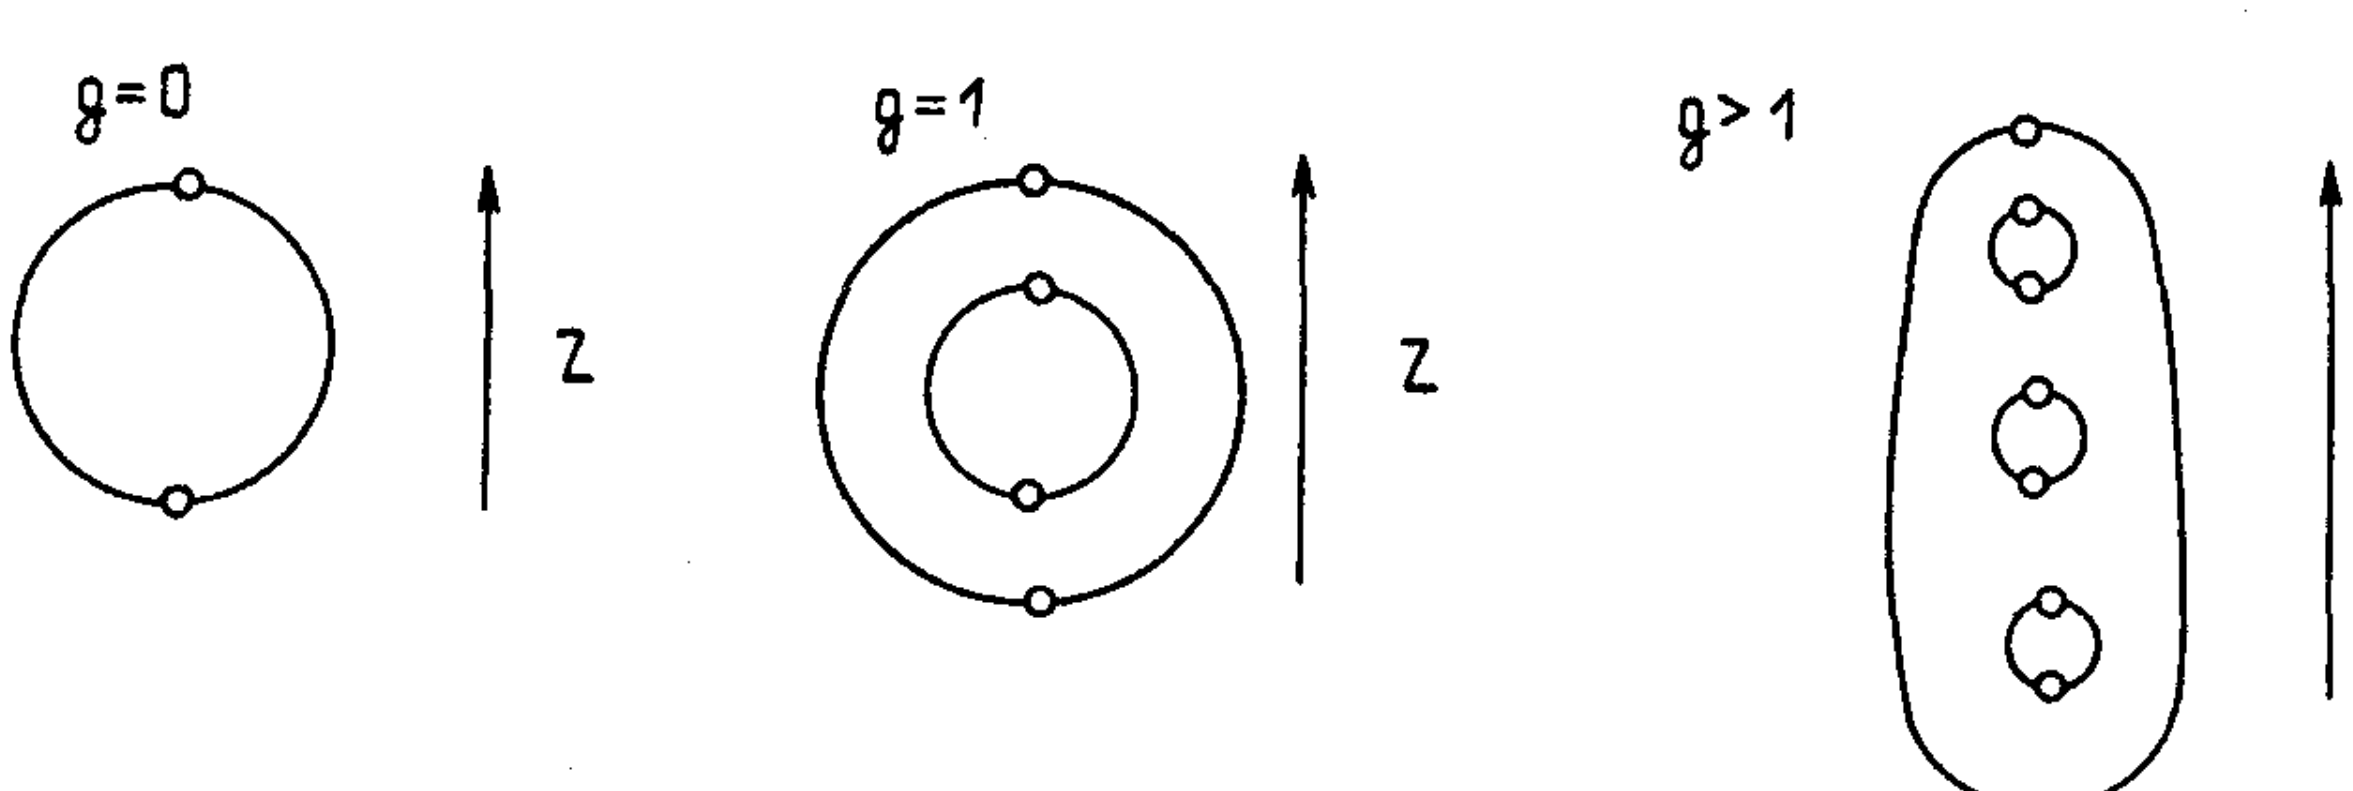
\includegraphics[width=0.80\textwidth]{figures/fig4_9.png}
  \figtitle{4.9}{}
\end{figure}

注意，流形 $M^n$ 上的 Morse 函数总可以取得使对 $f$ 的任一临界值 $c$，都存在 $\eps>0$，使 $f^{-1}[c-\eps,c+\eps]$ 只含一个临界点 $x_0$，$f(x_0)=c$。若 $x_0$ 是这样一个指标为 $\lambda$ 的临界点，则流形
\[
  M^n_{c+\eps}\quad(f(x)\le c+\eps)\qquad\text{与}\qquad
  M^n_{c-\eps}\quad(f(x)\le c-\eps),
\]
及其边界
\[
  N^{n-1}_{c+\eps}\quad(f(x)=c+\eps)\qquad\text{与}\qquad
  N^{n-1}_{c-\eps}\quad(f(x)=c-\eps),
\]
之间有如下联系：考虑「指标为 $\lambda$ 的 $n$ 维把手」
\[
  H^n_\lambda=D^{n-\lambda}\times D^\lambda,
\]
其边界为
\[
  \partial H^n_\lambda=(S^{n-\lambda-1}\times D^\lambda)\cup(D^{n-\lambda}\times S^{\lambda-1}).
\]
把边界 $\partial H^n_\lambda$ 的部分 $D^{n-\lambda}\times S^{\lambda-1}$ 与 $N^{n-1}_{c-\eps}=\partial M^n_{c-\eps}$ 中某个嵌入的 $(\lambda-1)$-球面的适当小管状邻域通过微分同胚
\[
  \psi:D^{n-\lambda}\times S^{\lambda-1}\longrightarrow N^{n-1}_{c-\eps}
\]
等同起来。

% [原文 p.171]
然后把把手 $H^n_\lambda$ 经微分同胚 $\psi$ 贴附到 $M^n_{c-\eps}$ 上，并把「角」磨光，得到光滑带边流形。可以证明，这样做可使所得流形与 $M^n_{c+\eps}$ 微分同胚，即得到
\[
  M^n_{c+\eps}\cong M^n_{c-\eps}\cup_\psi (D^{n-\lambda}\times D^\lambda).
\]
这一过程诱导出「Morse 手术」
\[
  N^{n-1}_{c-\eps}\longmapsto N^{n-1}_{c+\eps},
\]
其中
\[
  N^{n-1}_{c+\eps}\cong\Bigl(N^{n-1}_{c-\eps}\setminus\bigl(\tilde{D}^{n-\lambda}\times S^{\lambda-1}\bigr)\Bigr)
  \cup_\psi (S^{n-\lambda-1}\times D^\lambda).
\]
（这里 $\tilde{D}^{n-\lambda}$ 表示圆盘 $D^{n-\lambda}$ 的内部。）

\begin{figure}[htbp]
  \centering
  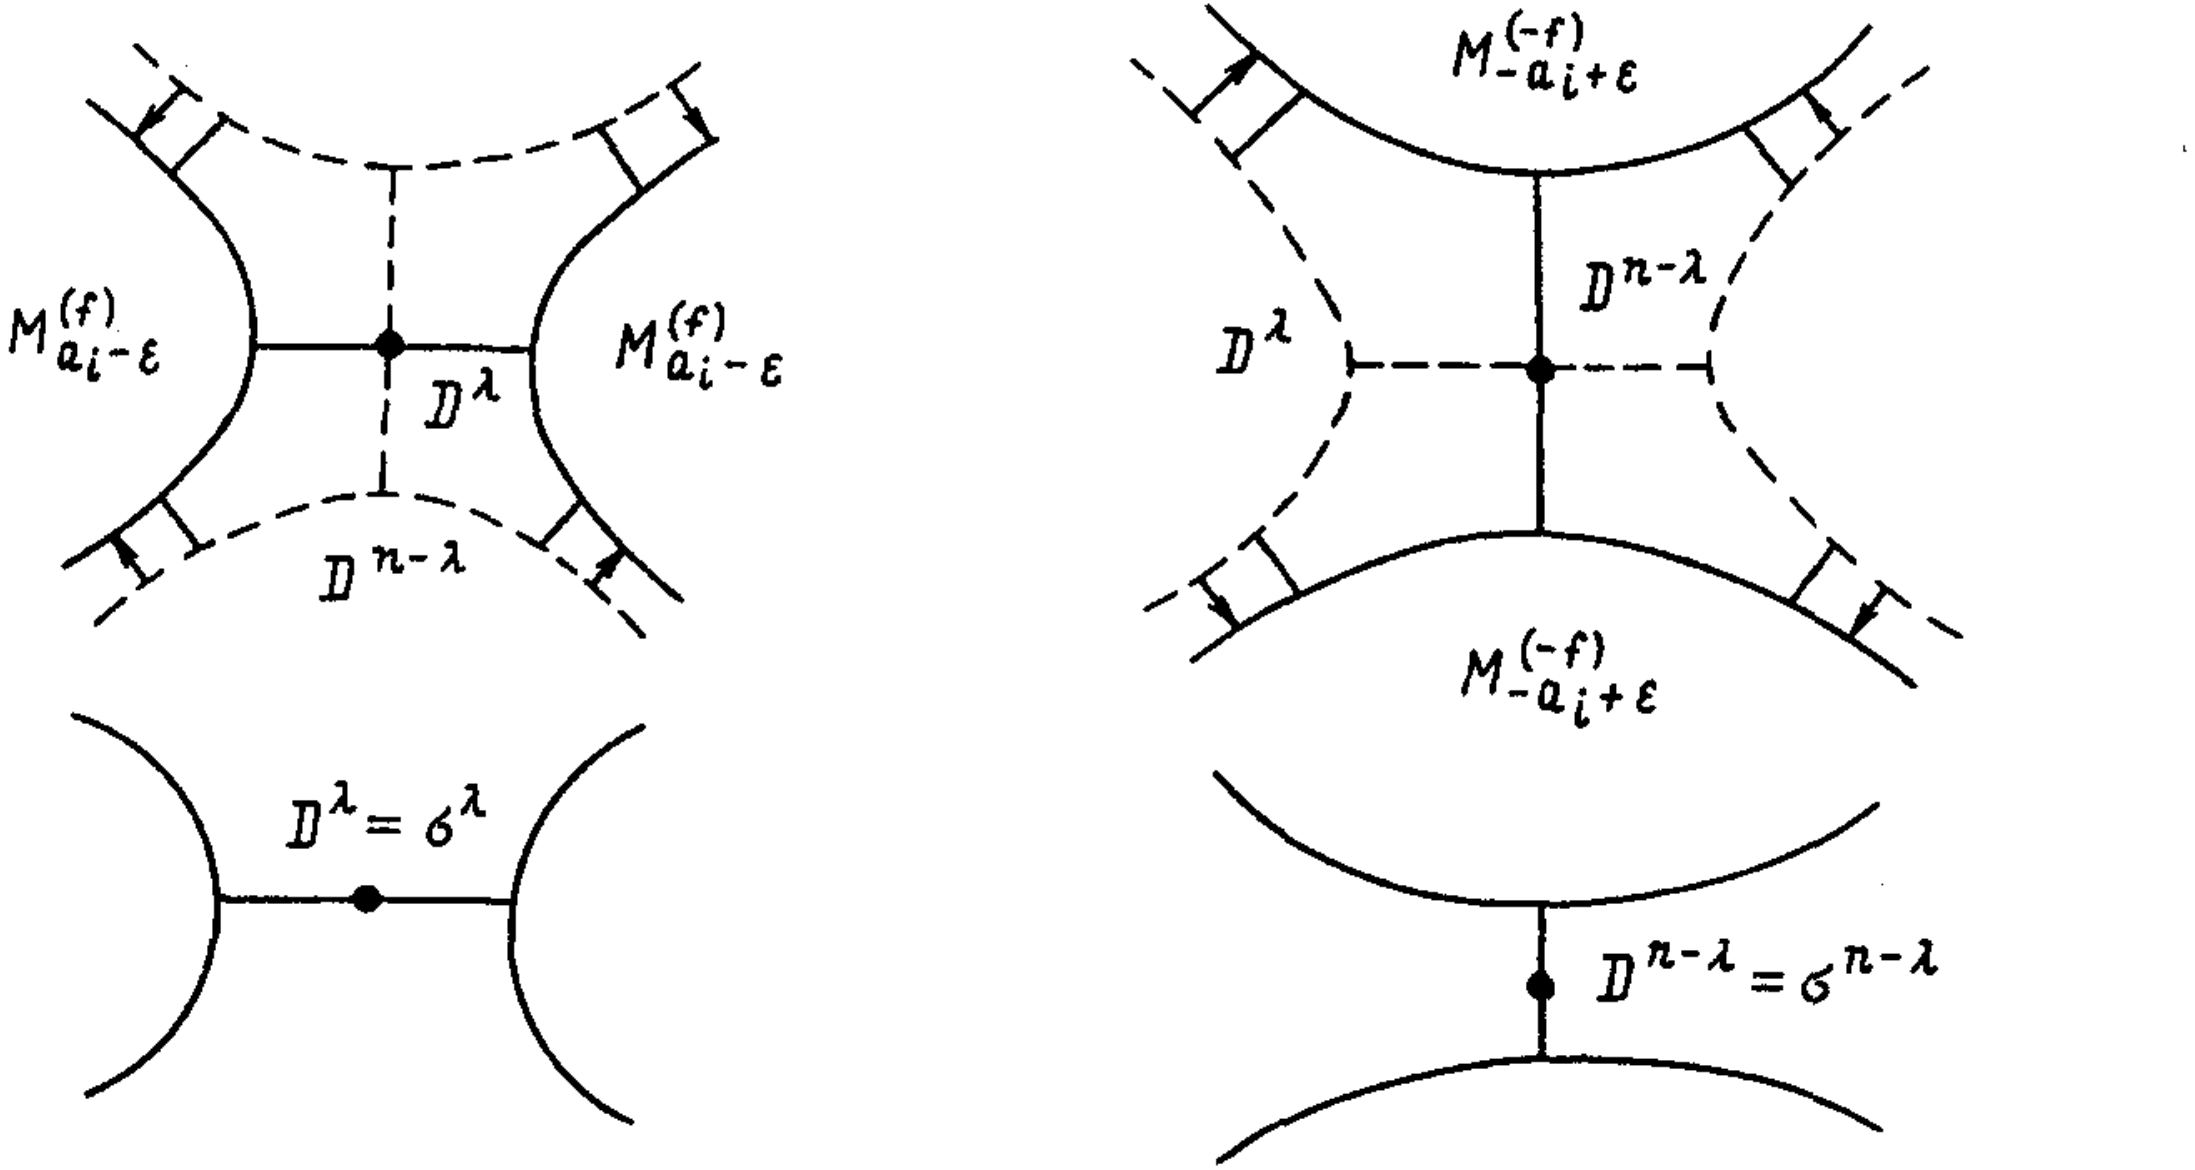
\includegraphics[width=0.86\textwidth]{figures/fig4_10.png}
  \figtitle{4.10}{}
\end{figure}
% [Tutor Note: 图 4.10 左右两半分别是 f 与 -f 的把手，指标互补为 n。Morse 手术切除的是 int D^{n-lambda} 乘 S^{lambda-1}，其边界为 S^{n-lambda-1} 乘 S^{lambda-1}；再用 S^{n-lambda-1} 乘 D^lambda 沿此边界粘上，粘合面维数为 n-2。]

于是 $M^n$ 上的 Morse 函数给出流形 $M^n$ 的「把手分解」，即把流形分解为把手的「和」。（图 4.11 显示把指标为 1 的二维把手 $H^2_1$ 贴附到圆盘 $H^2_0$ 上的两种可能；图 4.12 则用「Smale 函数」（即临界值按指标顺序排列的 Morse 函数），从 $H^2_0$ 出发，每越过一个临界点就贴附一个把手，对环面施行 Morse 手术。）

Morse 定理给出闭流形 $M^n$ 上 Morse 函数 $f$ 的指标为 $\lambda$ 的临界点个数 $m_\lambda$ 的如下下界估计，把这个数目与 $M^n$ 的整同调联系起来：

% [原文 p.172]
\begin{figure}[htbp]
  \centering
  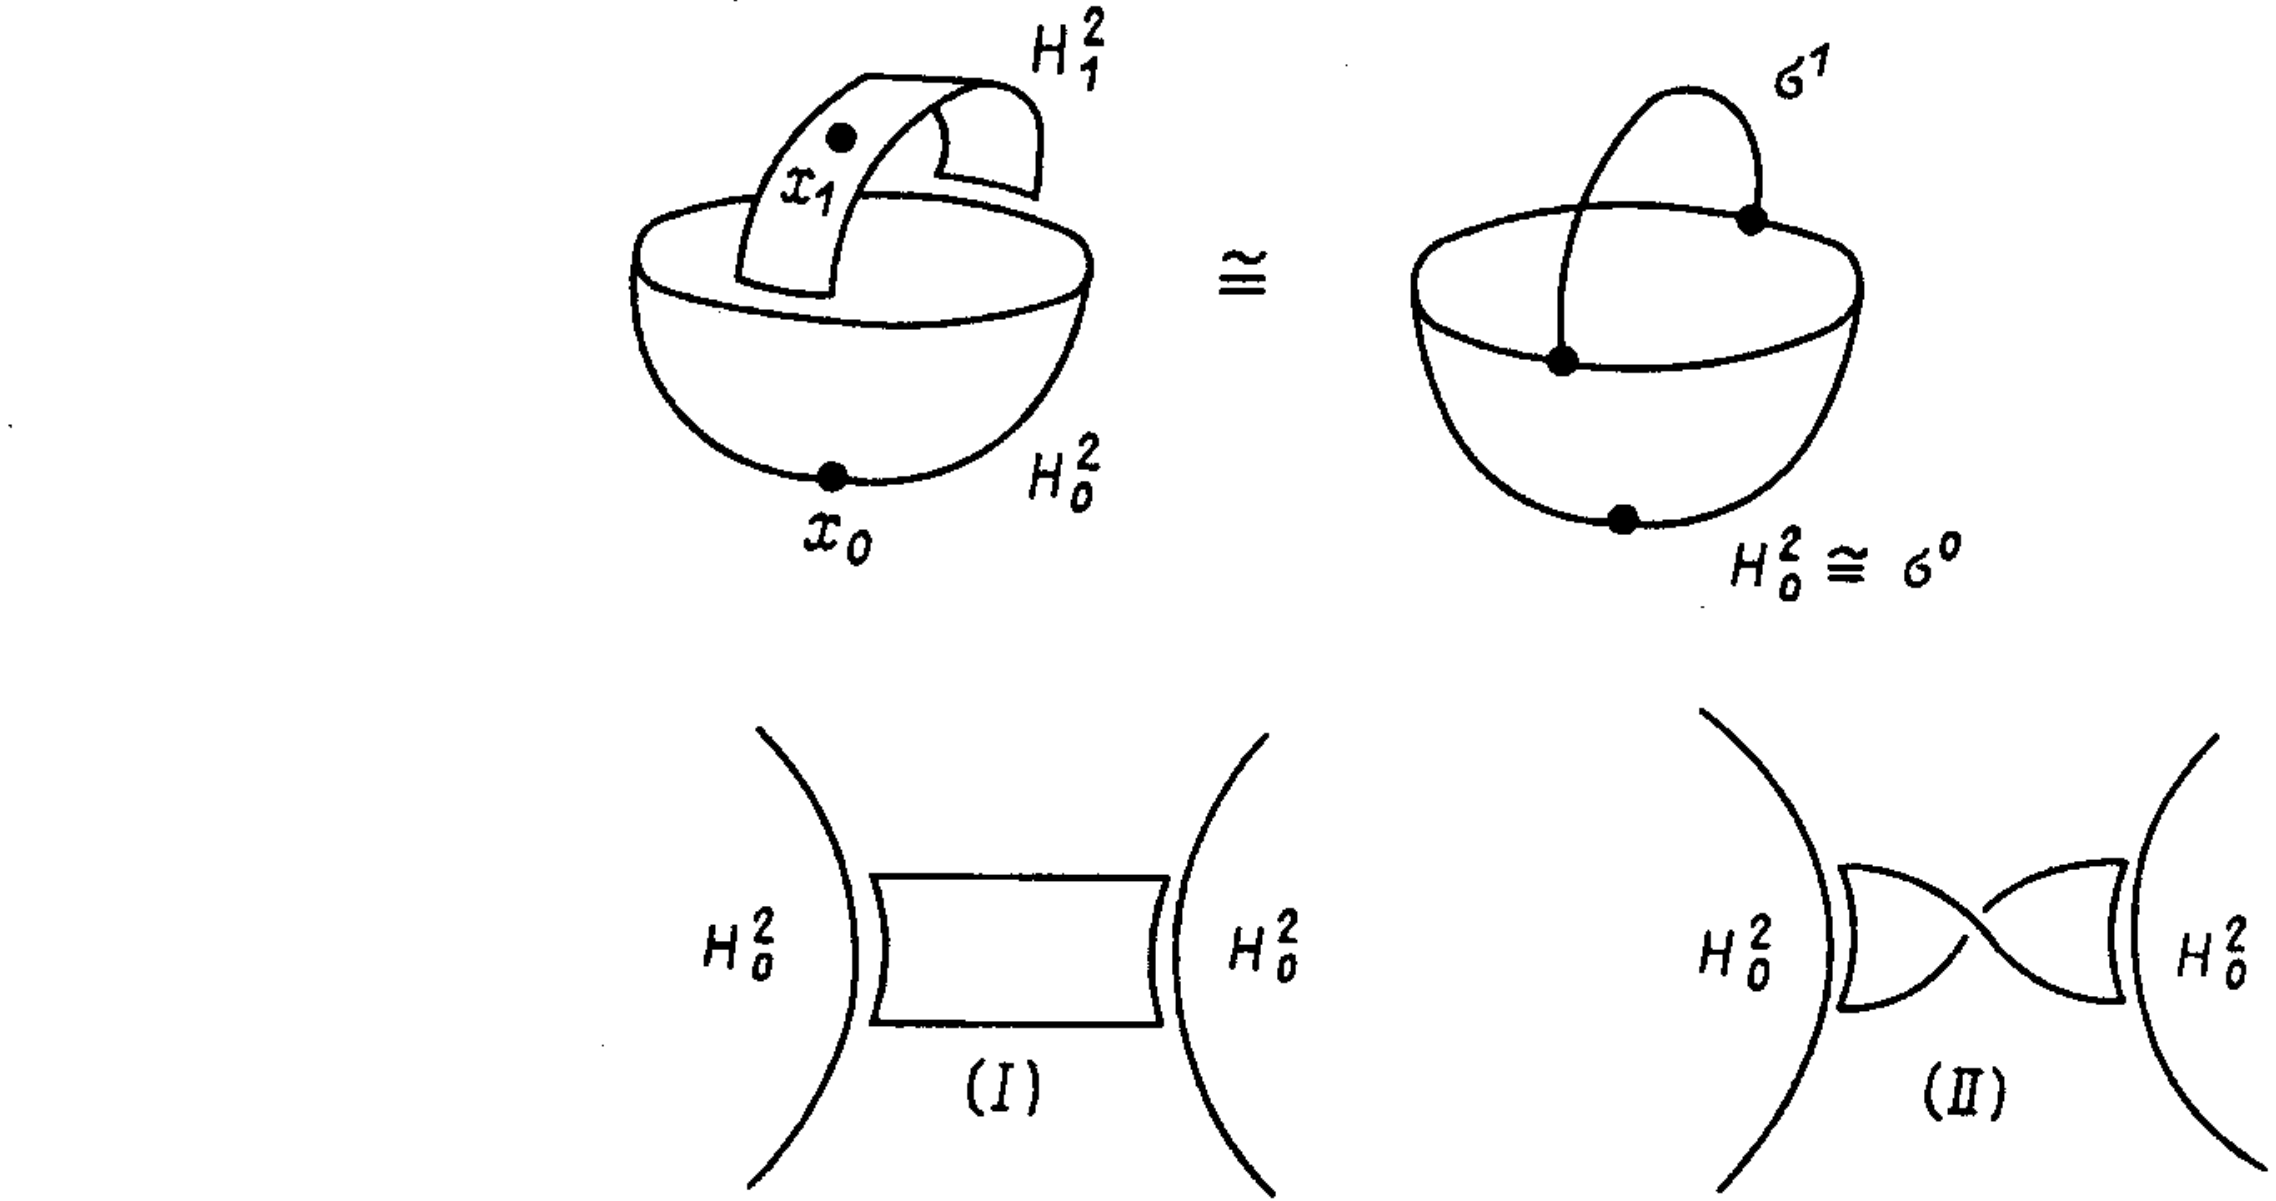
\includegraphics[width=0.86\textwidth]{figures/fig4_11.png}
  \figtitle{4.11}{}
\end{figure}

\begin{equation}
  m_\lambda(f)\ge b_\lambda,\qquad m_\lambda(f)\ge b_\lambda^{(p)}, \tag{2.8}
\end{equation}
其中 $b_\lambda$ 是第 $\lambda$ 个 Betti 数（$=\rank H_\lambda(M^n;\Z)$），$b_\lambda^{(p)}$ 是第 $\lambda$ 个 mod $p$ Betti 数（见第 3 章 §2）。

记 $q_\lambda$ 为 $H_\lambda(M^n;\Z)$ 的挠子群 $\Tor H_\lambda(M^n;\Z)$ 的最少生成元个数。由不同系数群下同调群之间的关系（见第 3 章 §2）可推出
\begin{equation}
  m_\lambda(f)\ge b_\lambda+q_\lambda+q_{\lambda-1}. \tag{2.9}
\end{equation}
这些就是 \emph{Morse 不等式}。

\begin{figure}[htbp]
  \centering
  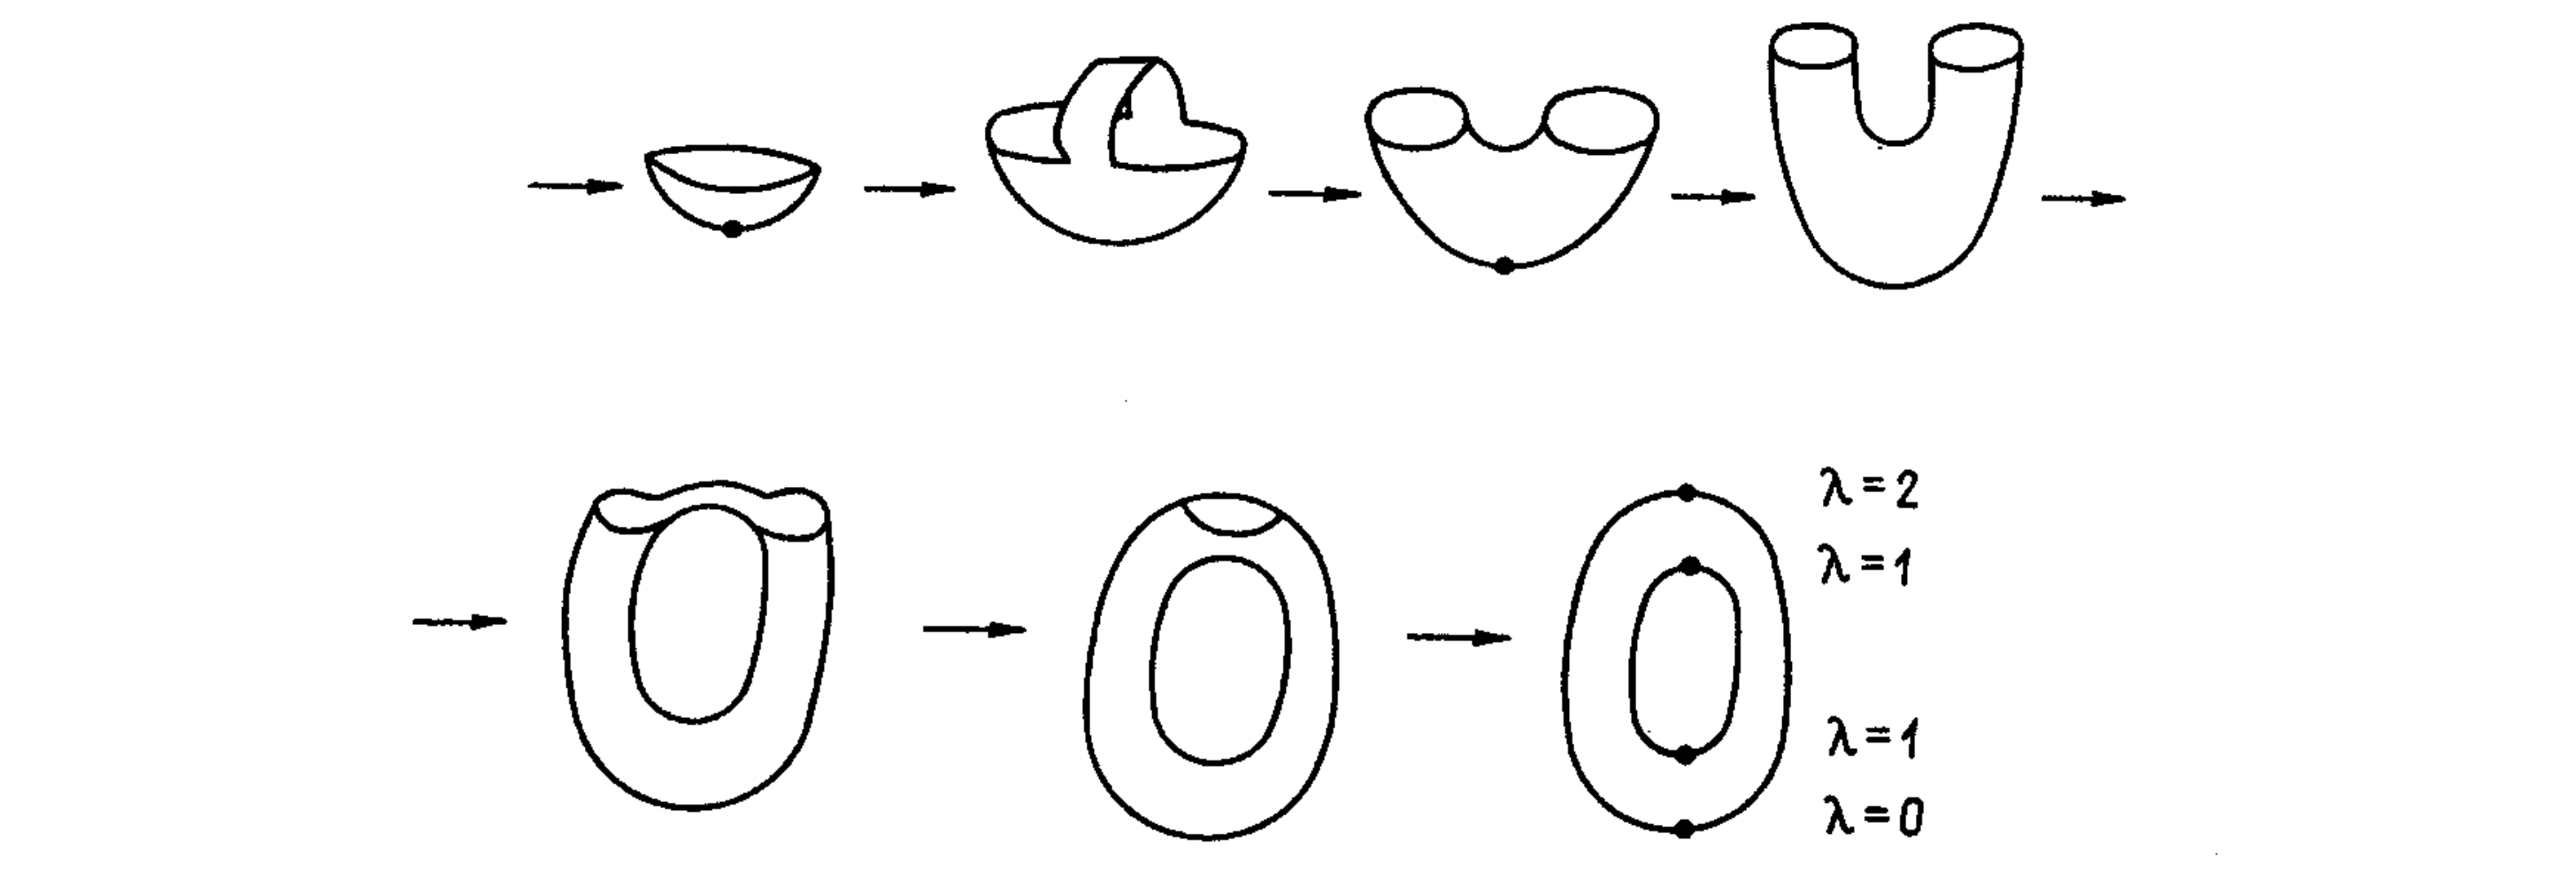
\includegraphics[width=0.86\textwidth]{figures/fig4_12.png}
  \figtitle{4.12}{}
\end{figure}

% [原文 p.173]
对维数不小于 6 的单连通流形，这些不等式是「严格的」，意思是：存在 $M^n$ 上的 Morse 函数 $f$，使式 (2.9) 中所有等式同时成立（Smale，20 世纪 60 年代初）。

闭流形 $M^n$ 上的 Morse 函数 $f$ 可用来构造与流形同伦等价的 $CW$-复形，其中每个维数 $\lambda$ 的胞腔个数恰为 $f$ 的指标为 $\lambda$ 的临界点个数。构造的基本想法如下：给 $M^n$ 配以 Riemann 度量 $g_{ij}$，考虑向量场 $-\mathrm{grad}\,f$，它在局部坐标 $\{x_\alpha^i\}$ 下局部地给出动力系统
\begin{equation}
  \frac{dx_\alpha^i}{dt}=-g^{ij}\frac{\partial f}{\partial x_\alpha^j}, \tag{2.10}
\end{equation}
其中 $g^{ij}g_{jq}=\delta^i_q$。

设 $x_0$ 是指标为 $\lambda$ 的临界点，$f(x_0)=c$；仍用 $M^n_{c-\eps}$、$M^n_{c+\eps}$ 分别表示由不等式 $f(x)\le c-\eps$、$f(x)\le c+\eps$ 确定的带边流形，其中 $\eps$ 充分小，使 $f^{-1}[c-\eps,c+\eps]$ 中除 $x_0$ 外没有别的临界点。在 $x_0$ 的邻域 $U$ 中取坐标系 $\{x^j\}$，使恒等式
\[
  f(x)=c-(x^1)^2-\cdots-(x^\lambda)^2+(x^{\lambda+1})^2+\cdots+(x^n)^2
\]
在整个 $U$ 上对 Morse 函数 $f$ 成立。现在考虑 $\lambda$-圆盘的嵌入 $\phi:D^\lambda\to U$，它由公式
\[
  (x^1)^2+\cdots+(x^\lambda)^2\le\eps\qquad\text{与}\qquad
  x^{\lambda+1}=0,\ \ldots,\ x^n=0
\]
确定。

\begin{figure}[htbp]
  \centering
  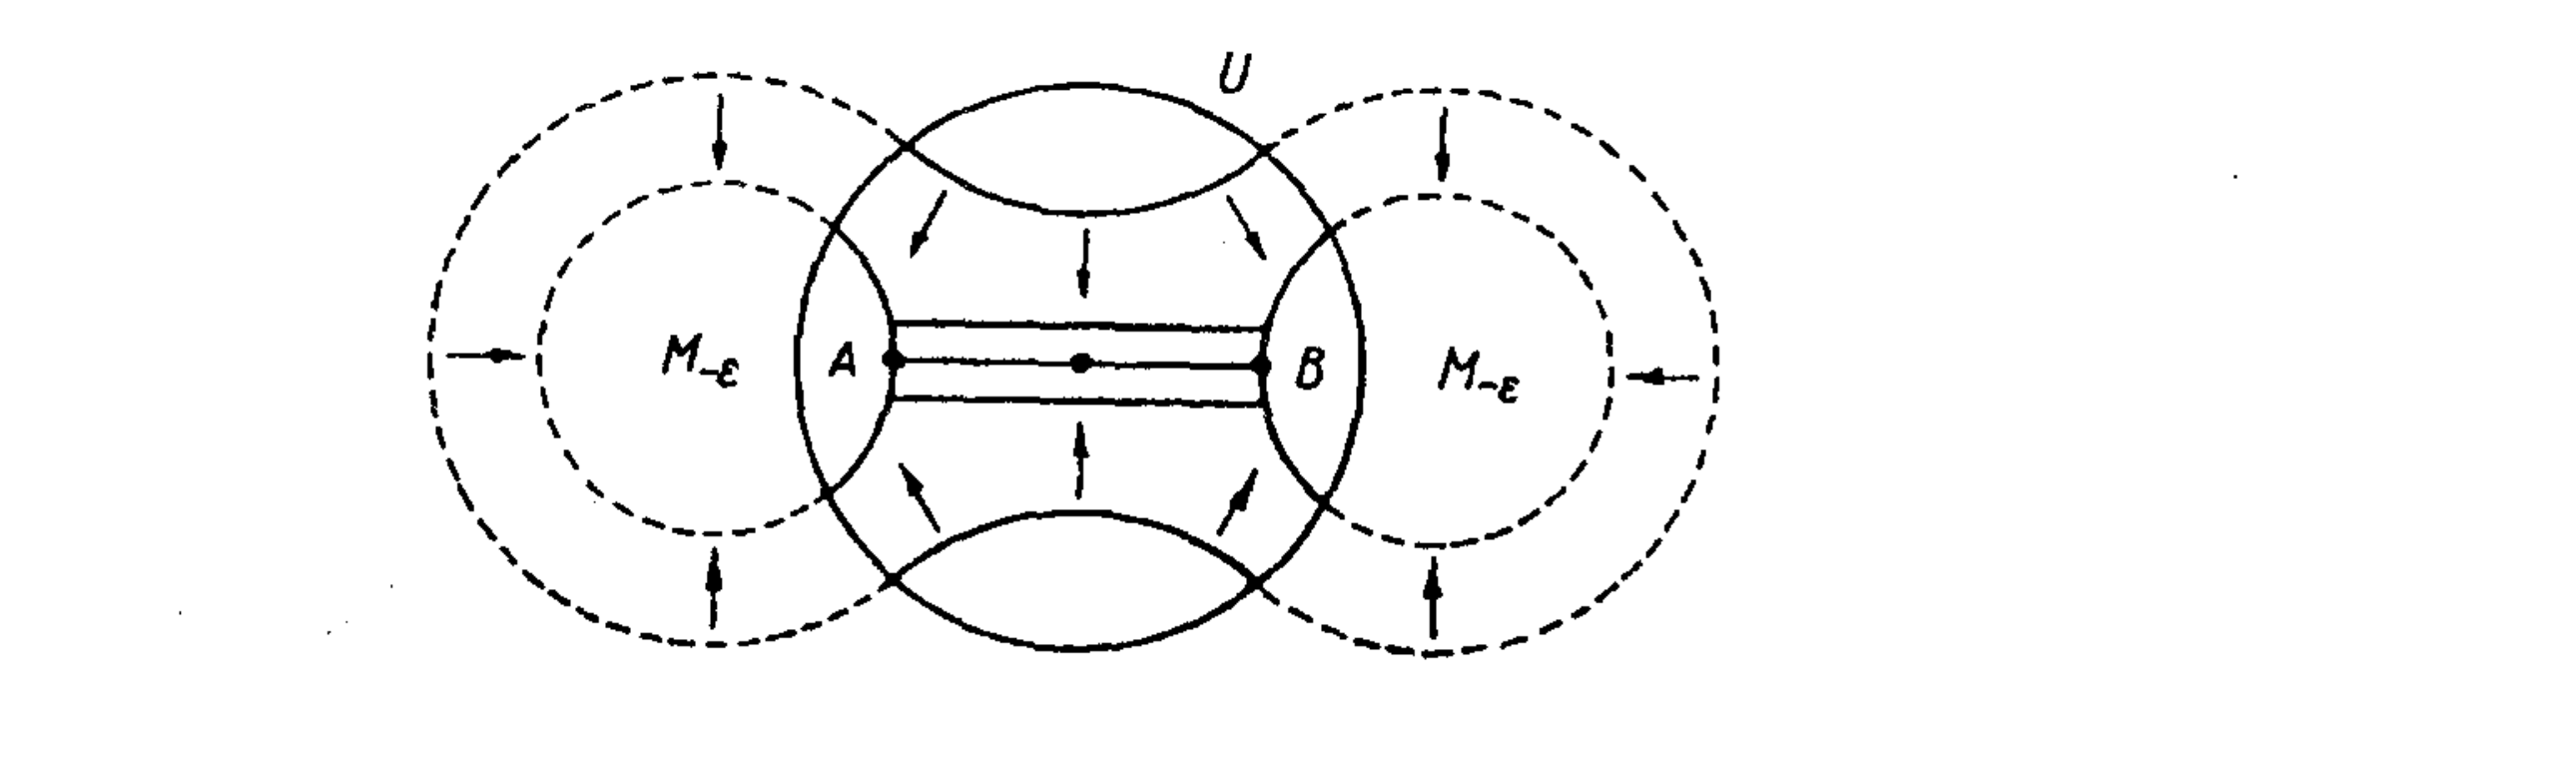
\includegraphics[width=0.86\textwidth]{figures/fig4_13.png}
  \figtitle{4.13}{}
\end{figure}

注意：
(i) $\phi(0)=x_0$；
(ii) $D^\lambda$ 上的函数 $\phi^*f$ 以圆盘中心为唯一（非退化）临界点（极大点）；

% [原文 p.174]
(iii) 边界 $\partial D^\lambda=S^{\lambda-1}$ 的像 $\phi(\partial D^\lambda)$ 包含在流形 $\partial M^n_{c-\eps}=\{x\in M^n\mid f(x)=c-\eps\}$ 中。

流形 $M^n_{c+\eps}$ 同伦等价于空间 $M^n_{c-\eps}\cup_\phi D^\lambda$。如下定义适当的同伦 $\varphi_\tau:M^n_{c+\eps}\to M^n_{c+\eps}$，$0\le\tau\le1$：在 $M^n_{c-\eps}$ 上它对所有 $\tau$ 都是恒等映射；在 $U$ 与 $M^n_{c-\eps}$ 之外，$\varphi_\tau$ 是 $M_{c+\eps}$ 的形变，它让点沿动力系统 (2.10) 的积分轨道（横截于水平面）移动。可以证明，在 $U$ 上同伦 $\varphi_\tau$ 可定义成把水平面族 $f^{-1}[c-\eps,c+\eps]$ 位于 $U$ 中的部分形变到 $\lambda$ 维圆盘 $D^\lambda$ 上——见图 4.13。要点在于：$\varphi_\tau$ 给出恒等映射 $\varphi_0:M_{c+\eps}\to M_{c+\eps}$ 与所需映射 $\varphi_1:M_{c+\eps}\to M^n_{c-\eps}\cup_\phi D^\lambda$ 之间的同伦。

对每个临界点依次施行这一构造，就得到与 $M^n$ 同伦等价的所需 $CW$-复形。每一步都可以通过把 $\varphi_1$ 作小扰动使之处于「一般位置」来保证：边界 $\partial D^\lambda$ 只贴附到已在 $M_{c-\eps}$ 中构造好的、维数小于 $\lambda$ 的胞腔上。（也可以改用 Smale 函数，即临界值的顺序与相应临界点指标的顺序一致的 Morse 函数。）

Morse 不等式（见上）很快可由这一与 $M^n$ 同伦等价的 $CW$-复形的构造推出。事实上它们还可补充：由该构造可推出
\begin{equation}
  \sum_{j=0}^{k}(-1)^jm_j(f)\ge\sum_{j=0}^{k}(-1)^jb_j, \tag{2.11}
\end{equation}
于是特别地取 $k=n$，得
\begin{equation}
  \sum_{j=0}^{n}(-1)^jm_j(f)=\chi(M^n). \tag{2.12}
\end{equation}
% [Tutor Note: (2.11) 的来由是 CW 复形 k-骨架的胞腔数交替和不超过全复形的交替和；取 k=n 时两侧都等于 Euler 示性数，因此 (2.12) 是恒等式，与 Morse 函数的选取无关。]

若闭流形 $M^n$ 上实值光滑函数的临界点孤立但允许退化，则 Morse 不等式不再适用。不过还有另一个有用的同伦不变量——流形的 Lyusternik--Shnirelman 范畴（20 世纪 20 年代末引入），它给出 $M^n$ 上光滑函数临界点个数的下界，而不论临界点是否非退化。对任意拓扑空间 $X$，该不变量记作 $\mathrm{cat}(X)$，定义为使 $X=\bigcup_i X_i$ 且每个 $X_i$ 在 $X$ 中可缩（可缩为一点）的闭集 $X_1,\ldots,X_k$ 的最少个数 $k$。于是有结论：对闭流形 $M^n$，$M^n$ 上任一光滑实值函数 $f$ 的临界点个数 $m(f)$ 满足
\[
  m(f)\ge\mathrm{cat}(M^n).
\]
反过来，$\mathrm{cat}(M^n)$ 又可用 $M^n$ 的上同调环（取适当系数）从下方估计：把 $M^n$ 的上同调
% [原文 p.175]
长度 $l(M^n)$ 定义为最大的 $l$，使得存在 $H^*(M^n;\Z)$（$M^n$ 不可定向时改用 $H^*(M^n;\Z/2)$）中正次数元素 $\alpha_1,\ldots,\alpha_l$ 的非零乘积 $\alpha_1\cdots\alpha_l$，则
\[
  \mathrm{cat}(M^n)>l(M^n).
\]
恒有 $\mathrm{cat}(M^n)\le n+1$。不难看出 $\mathrm{cat}(S^n)=2$；对 $S^2$ 以外的每个闭曲面 $M^2$ 有 $\mathrm{cat}(M^2)=3$；并且 $\mathrm{cat}(\RP^n)=n+1$，$\mathrm{cat}(\CP^n)=n+1$。以后我们将在变分法中出现的某些道路空间里考察 Morse 型和 Lyusternik--Shnirelman 型不等式。

最后，我们考虑流形 $M^n$ 上临界点构成 $M^n$ 的子流形的那种光滑函数 $f$；当 $M^n$ 存在 Lie 群对称性、且要求 $f$ 的水平集在该 Lie 作用下不变时，这类函数必然出现（见图 4.14）。

\begin{figure}[htbp]
  \centering
  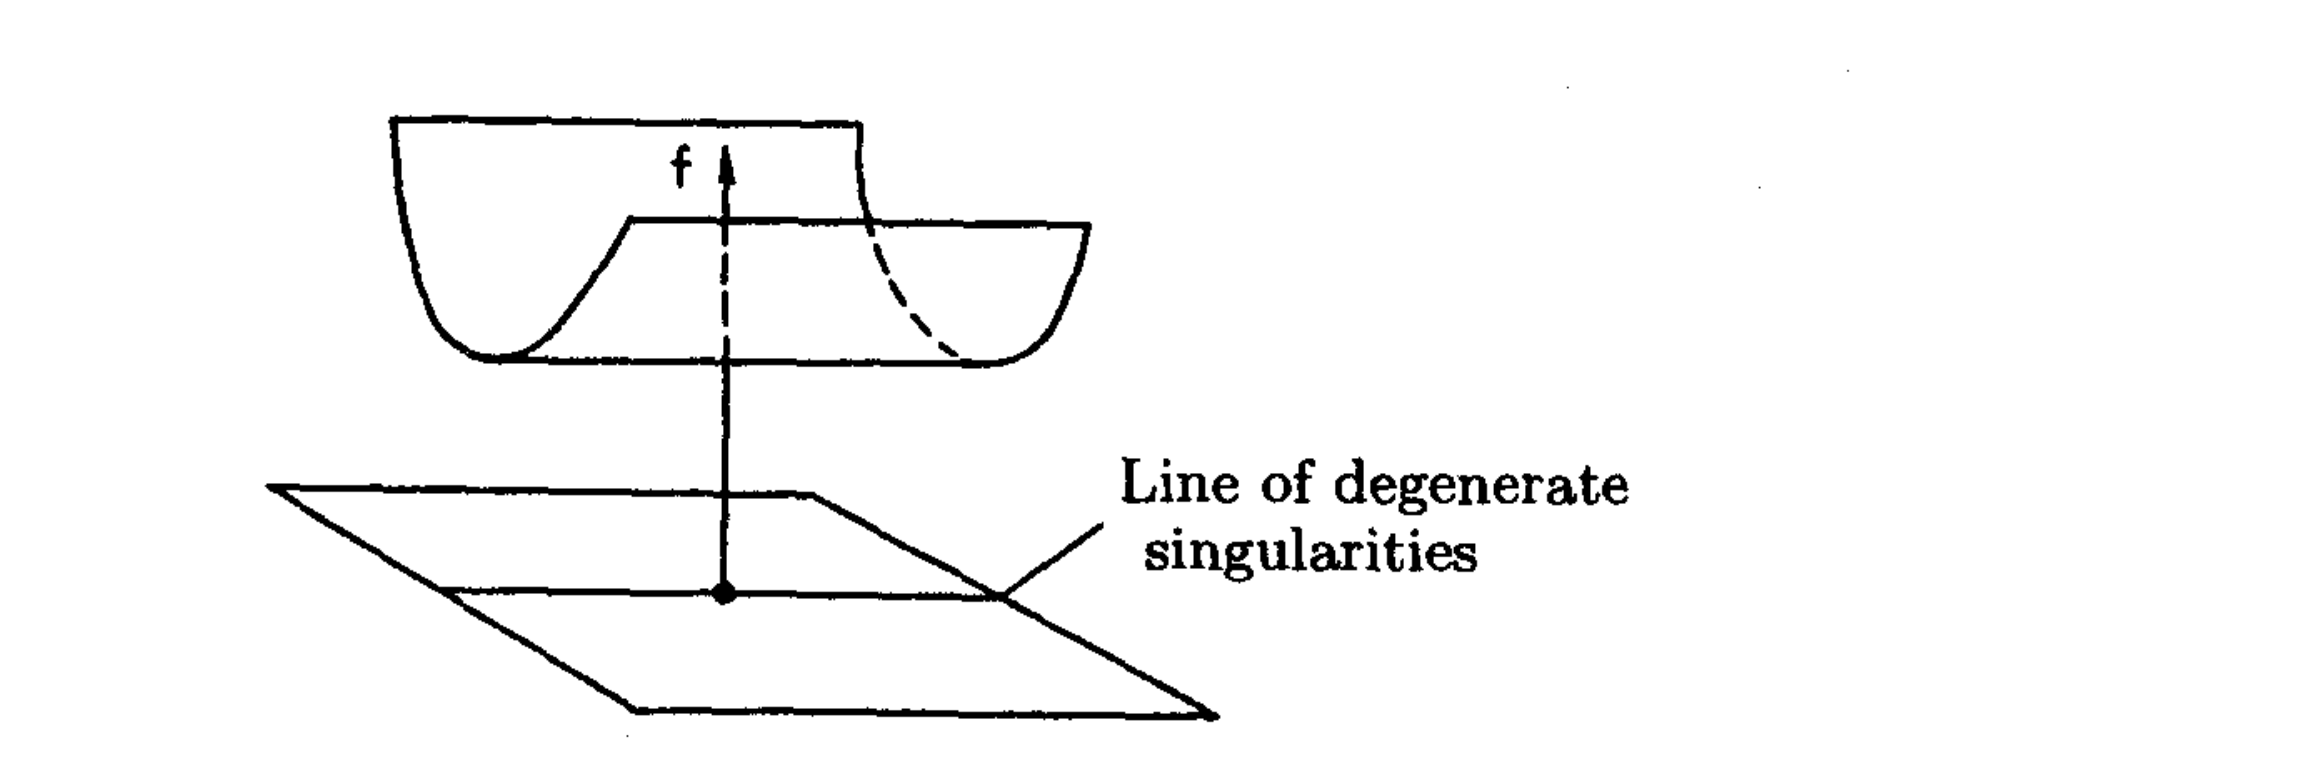
\includegraphics[width=0.86\textwidth]{figures/fig4_14.png}
  \figtitle{4.14}{}
\end{figure}

设 $f$ 是 $M^n$ 上的光滑函数。子流形 $W^k$ 称为 \emph{临界子流形}，若 $\mathrm{grad}\,f|_{W^k}\equiv0$。注意 Hessian $d^2f$ 在关于某个 Riemann 度与 $W^k$ 正交的子空间 $V^{n-k}_x\subset TM^n_x$ 上确定一个二次型。连通临界子流形 $W^k$ 称为 \emph{指标为 $\lambda$ 的非退化临界子流形}，若对任一 $x\in W^k$，二次型 $d^2f|_{V^{n-k}_x}$ 非退化且指标为 $\lambda$。（因 $W^k$ 连通，指标与点 $x$ 无关。）临界流形的特例由 Pontryagin 在 20 世纪 30 年代末结合 Lie 群 mod 2 Betti 数的计算考察过；一般理论及其最重要的应用则归功于 Bott（20 世纪 50 年代）。

在临界子流形 $W^k_\alpha\subset M^n$ 上自然定义向量丛 $\nu^{\lambda_\alpha}\to W^k_\alpha$，其纤维 $\R^{\lambda_\alpha}_x$ 由每点 $x\in W^k_\alpha$ 处的「最速下降」（即 $f$ 减小）方向给出，即由 Hessian $d^2f$ 限制在 $W^k_\alpha$ 的法丛上所得的负平方项决定。

现在设方程 $\mathrm{grad}\,f=0$ 的解集构成 $M^n$ 的一族光滑临界子流形 $W^k_\alpha$，指标为 $\lambda_\alpha$。若对每个 $W^k_\alpha$，刚才定义的向量丛 $\nu^{\lambda_\alpha}\to W^k_\alpha$ 可定向（即

% CHUNK ch04c DONE
